% This is samplepaper.tex, a sample chapter demonstrating the
% LLNCS macro package for Springer Computer Science proceedings;
% Version 2.20 of 2017/10/04
%
\documentclass[runningheads]{llncs}
%
\usepackage{graphicx}
% Used for displaying a sample figure. If possible, figure files should
% be included in EPS format.
%\usepackage{tikz}
%\usetikzlibrary{arrows}
\usepackage{verbatim}
%\usepackage{amsmath}
%\usepackage{amssymb}
%\usepackage{graphicx}
%\usepackage[all]{xy}
\usepackage{array}
\usepackage{enumitem}
%\usepackage{cite}
\usepackage{natbib}
% If you use the hyperref package, please uncomment the following line
% to display URLs in blue roman font according to Springer's eBook style:
% \renewcommand\UrlFont{\color{blue}\rmfamily}
\usepackage[breaklinks=true]{hyperref}
\usepackage{breakcites}
\renewcommand\UrlFont{\color{blue}\rmfamily}

\usepackage{xcolor}
\usepackage{listings}
\definecolor{dkgreen}{RGB}{0,70,70}
\definecolor{ltblue}{RGB}{0,130,130}
\definecolor{dkviolet}{RGB}{140,0,210}
\definecolor{dkblue}{RGB}{0,0,140}
\definecolor{dkred}{RGB}{140,20,0}
\definecolor{dkorange}{RGB}{130,70,0}

% lstlisting coq style (inspired from a file of Assia Mahboubi)
\lstdefinelanguage{Coq}{ 
    % Anything betweeen $ becomes LaTeX math mode
    mathescape=true,
    % Comments may or not include Latex commands
    texcl=false, 
    % Vernacular commands
    morekeywords=[1]{Section, Module, End, Require, Import, Export,
        Variable, Variables, Parameter, Parameters, Axiom, Hypothesis,
        Hypotheses, Notation, Local, Tactic, Reserved, Scope, Open, Close,
        Bind, Delimit, Definition, Let, Ltac, Fixpoint, CoFixpoint, Add,
        Morphism, Relation, Implicit, Arguments, Unset, Contextual,
        Strict, Prenex, Implicits, Inductive, CoInductive, Record,
        Structure, Canonical, Coercion, Context, Class, Global, Instance,
        Program, Infix, Theorem, Lemma, Corollary, Proposition, Fact,
        Remark, Example, Proof, Goal, Save, Qed, Defined, Hint, Resolve,
        Rewrite, View, Search, Show, Print, Printing, All, Eval, Check,
        Projections, inside, outside, Def},
    % Gallina
    morekeywords=[2]{forall, exists, exists2, fun, fix, cofix, struct,
        match, with, end, as, in, return, let, if, is, then, else, for, of,
        nosimpl, when},
    % Sorts
    morekeywords=[3]{Type, Prop, Set, true, false, option},
    % Various tactics, some are std Coq subsumed by ssr, for the manual purpose
    morekeywords=[4]{pose, set, move, case, elim, apply, clear, hnf,
        intro, intros, generalize, dependent, constructor, subst, rename, pattern, after, destruct, induction, using, refine, inversion, injection, rewrite, congr, unlock, compute, ring, field, fourier, replace, fold, unfold,
        change, cutrewrite, simpl, have, suff, wlog, suffices, without,
        loss, nat_norm, assert, cut, trivial, revert, bool_congr, nat_congr,
        symmetry, transitivity, auto, split, left, right, autorewrite},
    % Terminators
    morekeywords=[5]{by, done, exact, reflexivity, tauto, romega, omega,
        assumption, solve, contradiction, discriminate},
    % Control
    morekeywords=[6]{do, last, first, try, idtac, repeat},
    % Comments delimiters, we do turn this off for the manual
    morecomment=[s]{(*}{*)},
    % Spaces are not displayed as a special character
    showstringspaces=false,
    % String delimiters
    morestring=[b]",
    morestring=[d],
    % Size of tabulations
    tabsize=3,
    % Enables ASCII chars 128 to 255
    extendedchars=false,
    % Case sensitivity
    sensitive=true,
    % Automatic breaking of long lines
    breaklines=false,
    % Default style fors listings
    basicstyle=\small,
    % Position of captions is bottom
    captionpos=b,
    % flexible columns
    columns=[l]flexible,
    % Style for (listings') identifiers
    identifierstyle={\ttfamily\color{black}},
    % Style for declaration keywords
    keywordstyle=[1]{\ttfamily\color{dkblue}},
    % Style for gallina keywords
    keywordstyle=[2]{\ttfamily\color{dkgreen}},
    % Style for sorts keywords
    keywordstyle=[3]{\ttfamily\color{ltblue}},
    % Style for tactics keywords
    keywordstyle=[4]{\ttfamily\color{dkorange}},
    % Style for terminators keywords
    keywordstyle=[5]{\ttfamily\color{dkred}},
    %Style for iterators
    keywordstyle=[6]{\ttfamily\color{dkviolet}},
    % Style for strings
    stringstyle=\ttfamily,
    % Style for comments
    commentstyle={\ttfamily\color{dkgreen}},
    %moredelim=**[is][\ttfamily\color{red}]{/&}{&/},
    literate=
    {forall}{{$\forall\;$}}1
    {exists}{{$\exists\;$}}1
    {\\subsetOf}{{$\subseteq\;$}}1
    {<-}{{$\leftarrow\;$}}1
    {=>}{{$\Rightarrow\;$}}1
    {==}{{\code{==}\;}}1
    {==>}{{\code{==>}\;}}1
    %    {:>}{{\code{:>}\;}}1
    {->}{{$\rightarrow\;$}}1
    {<->}{{$\leftrightarrow\;$}}1
    {<==}{{$\leq\;$}}1
    {\#}{{$^\star$}}1 
    {\\o}{{$\circ\;$}}1 
    {\@}{{$\cdot$}}1 
    {\/\\}{{$\wedge\;$}}1
    {\\\/}{{$\vee\;$}}1
    %{++}{{\code{++}}}1
    {~}{{$\neg$}}1
    {<>}{{$\neq$ }}1
    {\@\@}{{$@$}}1
    {\\mapsto}{{$\mapsto\;$}}1
    {\\hline}{{\rule{\linewidth}{0.5pt}}}1
    %
}[keywords,comments,strings]

\begin{document}
%
\title{Contribution Title\thanks{Supported by organization x.}}
%
%\titlerunning{Abbreviated paper title}
% If the paper title is too long for the running head, you can set
% an abbreviated paper title here
%
\author{Sarah Johnson \and
Perry Alexander}
%
\authorrunning{S. Johnson and P. Alexander.}
% First names are abbreviated in the running head.
% If there are more than two authors, 'et al.' is used.
%
\institute{Institute for Information Sciences \\ The
  University of Kansas \\ Lawrence, KS 66045 \\
  \email{\{sarahjohnson,palexand\}@ku.edu}}
%
\maketitle              % typeset the header of the contribution
%
\begin{abstract}
%The abstract should briefly summarize the contents of the paper in 15--250 words.
A secure device identifier (DevID) is defined as an identifier that is cryptographically bound to a device. Trusted Platform Module (TPM) keys are an ideal choice for implementation of these identifiers.
The specification ``TPM 2.0 Keys for Device Identity and Attestation'' by the Trusted Computing Group (TCG) describes several procedures for remotely proving a key to be resident in a specific device's TPM and thereby satisfying the requirements for a DevID. These procedures are carefully constructed protocols that are intended to be performed by a trusted Certificate Authority (CA) in communication with a certificate-requesting device and are designed to maintain a cryptographic evidentiary chain linking a DevID to a specific TPM. The TCG claims that each protocol provides certain assurances; these assurances are the basis for the resulting cryptographic evidentiary chain. 
\textit{I aim to determine the correctness of these key certification protocols by abstractly modeling them and formally verifying their expected assurances}. I choose this goal since the TCG themselves do not provide proofs or clear justifications for how the protocols provide these assurances. 

\keywords{First keyword  \and Second keyword \and Another keyword.}
\end{abstract}
%
%
%
\section{Introduction}
Development and deployment of trusted systems often require definitive identification of devices. A remote entity should have confidence that a device is that which it claims to be. An ideal method for fulfulling this need is through the utilization of cryptographic keys in the Trusted Platform Module (TPM) as secure device identitifiers \citep{DevIDSpec-TCG}. A secure device identifier (DevID) is defined as an identifier that is cryptographically bound to a device \citep{DevIDSpec-IEEE}. 
A DevID must not be transferable from one device to another as that would allow distinct devices to be identified as the same. 
Since the TPM is a secure Root of Trust for Storage \citep{TPMSpec}, it provides the necessary protections for storing these identifiers and enforcing this constraint. 

The specification ``TPM 2.0 Keys for Device Identity and Attestation'' by the Trusted Computing Group (TCG) describes several procedures for remotely proving a key to be resident in a specific device's TPM \citep{DevIDSpec-TCG}. These procedures are carefully constructed protocols that are intended to be performed by a trusted Certificate Authority (CA) in communication with a certificate-requesting device. These protocols are designed to maintain a cryptographic evidentiary chain linking a DevID to a specific TPM \citep{DevIDSpec-TCG}. 
DevID certificates provisioned by an OEM at device manufacturing time should provide definitive evidence that a key belongs to a specific device. Whereas DevID certificates provisioned by a device owner require a chain of certificates in order to verify a chain of trust to an OEM-provided root certificate. This distinction is due to differences in the respective protocols prescribed by the TCG's specification. 
For each provisioning procedure described in the specification, the TCG outlines steps for the CA and the certificate-requesting entity to perform. Furthermore, the TCG claims that each procedure provides certain assurances. These assurances are the basis for the resulting cryptographic evidentiary chain.
Each assurance manifests as an assertion regarding either TPM-residency, key attributes, or previously-issued certificates.

This work places special emphasis on two key certification protocols, namely OEM Creation of an IAK Certificate based on an EK Certificate and Owner Creation of an LAK Certificate based on an IAK Certificate. I select these protocols due to their especially significant security and identity implications. \textit{The primary goal of this work is to determine the correctness of these two protocols by abstractly modeling them and formally verifying their expected assurances}. I choose this goal since the TCG themselves do not provide proofs or clear justifications for how the protocols provide these assurances. 
The contributions of the research presented in this thesis may be summarized as (1) a general investigation into TPM-based DevIDs and chains of certificates, (2) the design and implementation of an abstract formal model of command execution, (3) an in-depth analysis of two TCG-provided key certification protocols, and (4) the discovery of a potential shortcoming of the IAK provisioning procedure and consequently a recommendation for its improvement.

\section{Related Work}
The Privacy CA protocol of the TPM 1.2 has been extensively studied using various formal methods. The Privacy CA protocol was replaced by the Direct Anonymous Attestation (DAA) scheme in the TPM 2.0. Both of these protocols aim to accomplish the same fundamental purpose: allow remote authentication of a device while maintaining its anonymity. These protocols differ from the key certification protocols analyzed in my work which aim to provide individual identification of a device.
The work of Chen et al.\ \citep{PrivacyCAAnalysis-Chen} analyzes the Privacy CA protocol in the presence of an adversary. They suggest a small modification to the protocol that enhances its security without changing the existing functionality of the TPM 1.2. I similarly suggest a small modification to the IAK provisioning procedure which requires no change to the existing functionality of the TPM 2.0.
On the other hand, the work of Halling et al.\ \citep{PrivacyCAAnalysis-Hall,TPM12Model} analyzes the Privacy CA protocol but does not consider any specific adversary. Instead, they consider the functional correctness of the protocol and specifically examine the protocol implementation to ensure that it produces the results that it should.  
My work has many parallels to the works of Halling et al. 
I attempt to determine whether the implementations of certain key certification protocols result in the assurances that they should.
Furthermore, Halling et al.\ abstractly model a large subset of the TPM 1.2 commands in the PVS specification language. They model TPM command execution as a transition system over an abstract system state. I implement this same technique in my own work but over a small subset of TPM 2.0 commands as well as several non-TPM commands. 

The works of Whitefield et al.\ \citep{DAAAnalysis-Whit} and Wesemeyer et al.\ \citep{DAAAnalysis-Wes} thoroughly study the DAA scheme of the TPM 2.0. Collectively, they develop a symbolic model, a C++ implementation, and a formally-verified fix of the scheme. 
Many other works use formal methods to examine other aspects of both the TPM 1.2 \citep{AuthAnalysis,PCRAnalysis} and 2.0 \citep{EAAnalysis,HMACAnalysis}.
These aspects include authentication, platform configuration registers (PCRs), enhanced authorization (EA), and hash-based message authentication code (HMAC) mechanisms. They utilize tools and techniques such as SAPIC, Tamarin, stateful applied pi calculus, amongst others. 
%
%
%
\section{TPM 2.0}
A Trusted Platform Module (TPM) is a microcontroller that complies with the ISO/IEC 11889:2015 international standard.
The TPM and its specification were designed by the Trusted Computing Group (TCG) to act as a hardware anchor for PC system security. To this end, TPMs have the abilities necessary for secure generation of keys, algorithm agility, secure storage of keys, enhanced authorization, device health attestation, device identification, NVRAM storage and more \citep{{PracticalGuide}}. 

Device health attestation data provided by a TPM offers cryptographic proof of software state. Attestation data comes in the form of a quote which is a signed hash over a selection of platform configuration registers. Platform configuration registers (PCRs) store the results from a chain of boot time measurements in a way that guarantees integrity. In particular, a PCR cannot be rolled back to a previous value resulting in a measurement being undone. To tie attestation data to a specific device, the key that performed the signing operation must be cryptographically bound to that device, that is, the key must be a secure device identifier. 

A key may then be created using one of two commands.
\begin{itemize}
  \item \verb|TPM2_CreatePrimary|: A Primary key is produced based on the current Primary Seed. A Primary key may be persisted within the TPM. Otherwise it must be recreated after a TPM reset.
  \item \verb|TPM2_Create|: An Ordinary key is produced based on a seed taken from the RNG. An Ordinary key is the child of another key; it is wrapped by that parent key. It may be persisted within the TPM or persisted external to the TPM in the form of an encrypted key blob. The blob is only loadable using the parent key's authorization in the TPM that created it.
\end{itemize}
Keys have attributes that are set at creation-time. These attributes are permanent and include the following: \verb|FixedTPM|, \verb|Sign|, \verb|Decrypt|, and \verb|Restricted|. The \verb|FixedTPM| attribute indicates that the private key cannot be duplicated. A key pair with the \verb|Sign| attribute set consists of a private signing key and a public signature-verification key. When properly handled, private signing keys can provide integrity, authenticity, and nonrepudiation. A key pair with the \verb|Decrypt| attribute set consists of a public encryption key and a private decryption key. When properly handled, public encryption keys can provide confidentiality.
Our Coq model inductively defines a \verb|pubKey| and \verb|privKey| type for public keys and private keys respectively. A key of either type requires a unique identifier and a sequence of boolean values describing whether a particular attribute is set or not set. A key pair consists of a \verb|pubKey| and a \verb|privKey| with the same identifier and attributes.
\begin{figure}[h]
\begin{lstlisting}[language=Coq]
Inductive pubKey : Type :=
| Public : keyIdType -> Restricted -> Sign -> Decrypt -> FixedTPM -> pubKey.

Inductive privKey : Type :=
| Private : keyIdType -> Restricted -> Sign -> Decrypt -> FixedTPM -> privKey.
\end{lstlisting}

\caption{Model of Keys}
\end{figure}

The \verb|Restricted| attribute provides important security
implications. A restricted signing key may only sign a digest that has
been produced by the TPM. A restricted signing key is used during key
certification to prove that a new key is loaded on the same TPM as
itself. During attestation, a restricted signing key is used to prove
that a quote is the result of the PCR values within the same TPM as
itself. Additionally, a restricted signing key has the ability to sign
data supplied to the TPM externally by using the \verb|TPM2_Hash|
command. When used for this purpose, the hash operation is called a
signature hash.

A restricted decryption key is called a storage key. Only storage keys
can be used as parents to create or load child objects or to activate
credentials \citep{PracticalGuide}. All TPMs are shipped with an
essential storage key: the endorsement key (EK). The EK is installed
by the TPM manufacturer and stored in a shielded location on the
TPM. The corresponding EK certificate serves a significant role in the
creation of DevID certificates.

\section{Secure Device Identity}
A secure device identifier (DevID) is defined as an identifier that is cryptographically bound to a device \citep{DevIDSpec-IEEE}. A DevID must not be transferable from one device to another and must be stored in a way that protects it from modification. Since the TPM is a secure Root of Trust for Storage and protects keys against compromise, TPM keys are an ideal choice for DevIDs. 
The binding of a TPM key to a specific device instance is represented by a DevID certificate.
To know when and by whom DevIDs are created, it is useful to briefly consider a simplified version of the process for creating and distributing TPM-containing devices to end users.
\begin{enumerate}
  \item\label{ite:idTPM} TPM Manufacturers produce TPM chips according to the international standard. They provision each TPM chip with an EK certificate that binds the EK to a specific TPM. These chips are then distributed to the original equipment manufacturers (OEMs).
  \item\label{ite:idDevIni} OEMs produce devices (e.g., PCs) with these TPM chips integrated. They provision each TPM chip with one or more DevID certificates that bind a key to a specific device. These devices are then distributed to the end users (Owners).
  \item\label{ite:idDevLoc} Owners may optionally provision their TPM chip with one or more DevID certificates that bind a key to their specific device.
\end{enumerate} 

The provisioning of device identification in Steps \ref{ite:idDevIni}
and \ref{ite:idDevLoc} is the primary subject of this work.

The issuers of  certificates are known as Certificate Authorities (CAs). CAs are further identified by the creator of the keys that they certify (i.e., the CA that issues certificates for EKs is known as the TPM Manufacturer's CA, the CA that issues certificates for IAKs and IDevIDs is known as the OEM's CA, and the CA that issues certificates for LAKs and LDevIDs is known as the Owner's CA). All CAs should support a standard certificate transport protocol that provides confidentiality, integrity, and protection from replay attacks \citep{DevIDSpec-TCG}. These transport protocols are outside the scope of this paper. 

The term certificate specifically refers to an X.509 v3 digital certificate. 
A certificate contains a public key and identifying information and is
signed by a Certificate Authority. In our model, certificates are abstractly defined by the inductive \verb|signedCert| type. This type greatly simplifies the true implementation of a certificate and includes only a select few of the associated fields. A \verb|signedCert| requires a public key, an identifier, and a private key. An identifier is an abstract representation of a certificate's Subject field and may include information describing either the TPM or the device. The private key parameter denotes the key that performed the signature over the certificate.
\begin{figure}[h]
\begin{lstlisting}[language=Coq]
Inductive identifier : Type :=
| TPM_info : tpmInfoType -> identifier
| Device_info : deviceInfoType -> identifier.

Inductive signedCert : Type :=
| Cert : pubKey -> identifier -> privKey -> signedCert.
\end{lstlisting}
\caption{Model of Certificates}
\end{figure}

An EK certificate's Subject field in combination with other fields imparts various assertions regarding the security qualities and provenance of the TPM \citep{EKSpec}. 
Although the EK is not a DevID, these assertions allow the EK to serve a significant role in the provisioning of DevIDs.
Specifically, the EK certificate is used in the creation of an IAK certificate, the first and arguably most important certificate that identifies a device.
Proving that an IAK belongs to a specific device requires first binding the IAK to a specific TPM using the EK and then binding the TPM to a specific device. Due to this reliance, an IAK certificate even includes a field which references the associated EK certificate's serial number.

Trust for creation of a new DevID certificate is based on an existing certificate. Therefore, a chain of certificates can be used to verify a chain of trust to some trust anchor \citep{DevIDSpec-TCG}. Since IAK certificates provide definitive evidence that a key belongs to a specific device, an IAK certificate typically acts as this trust anchor and thus typically is the root node in a chain of certificates. In issuing an IAK certificate, the OEM's CA makes an assertion that is a primary security dependency for the provisioning of all future DevIDs. 
The Subject field of DevID certificates contains non-TPM device information such as device model and serial numbers. This information should be globally unique per device \citep{DevIDSpec-IEEE}. All certificates in a chain should have the same Subject field as the IAK certificate.

\begin{figure}[h]
  \begin{centering}
  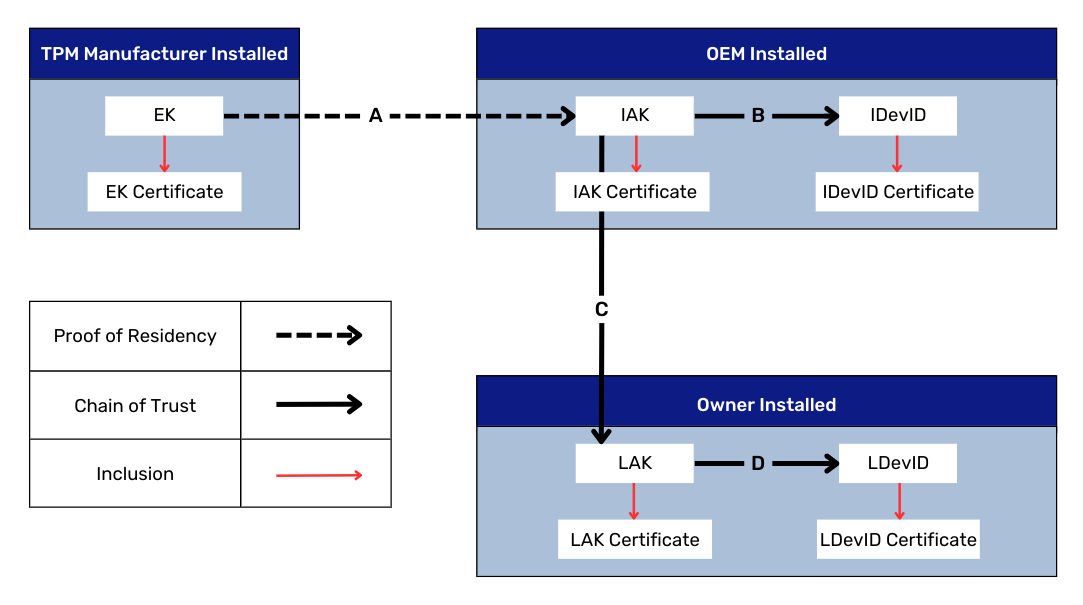
\includegraphics[width=\linewidth]{figures/certRelationships.png}
  \par\end{centering}
  \caption{Key and Certificate Relationships \citep{DevIDSpec-TCG}}
  \label{fig:cert_rel}
\end{figure}
\vspace{2em}
\begin{itemize}[itemsep=0pt,parsep=0pt,partopsep=0pt]
  \item \textsf{TPM Manufacturer Installed Box}: The EK certificate is signed by the TPM Manufacturer's CA and binds the EK to a specific TPM.
  \item \textsf{Line A}: The IAK is verified by the OEM's CA to have the correct key properties and to be loaded on the same TPM as the EK.
  \item \textsf{Line B}: The IDevID is verified by the OEM's CA to have the correct key properties and to be loaded on the same TPM as the IAK.
  \item \textsf{OEM Installed Box}: The IAK certificate and IDevID certificate is signed by the OEM's CA and binds the IAK and IDevID to a specific device.
  \item \textsf{Line C}: The LAK is verified by the Owner's CA to have the correct key properties and to be loaded on the same TPM as the IAK.
  \item \textsf{Line D}: The LDevID is verified by the Owner's CA to have the correct key properties and to be loaded on the same TPM as the LAK.
  \item \textsf{Owner Installed Box}: The LAK certificate and LDevID certificate is signed by the Owner's CA.
\end{itemize}

%
%
%
\section{Command Execution Model}
The protocols used to create DevID certificates require performing both TPM and non-TPM commands. A command may rely on a variety of parameters such as keys, nonces, certificates, as well as other messages. A message includes the structures that an entity may use or produce. The \verb|message| type is 
\begin{figure}[h]
\begin{lstlisting}[language=Coq]
Inductive message : Type :=
| publicKey : pubKey -> message
| privateKey : privKey -> message
| hash : message -> message
| signature : message -> privKey -> message
| TPM2B_Attest : pubKey -> message
| encryptedCredential : message -> randType -> pubKey -> message
| randomNum : randType -> message
| TCG_CSR_IDevID : identifier -> signedCert -> pubKey -> message
| TCG_CSR_LDevID : message -> signedCert -> message
| signedCertificate : signedCert -> message
| pair : message -> message -> message.
\end{lstlisting}
\caption{Model of Messages}
\end{figure}
an abstract representation of these structures. From a message, additional messages may be inferred. For example, given a message in the form \verb|signature m k|, the message \verb|m| may be deduced. Whereas given a message in the form \verb|encryptedCredential n g k|, no messages may be deduced. This concept is modeled in two ways: as a recursive function \verb|inferFrom| and as an inductive proposition \verb|inferrable|. These two definitions are proven equivalent and so may be used interchangeably. In particular, additional information may be gained from signatures, \verb|TPM2B_Attest| structures, certificate signing requests (CSRs), certificates, and pairs of messages. All other messages either contain no additional information (i.e., keys and random numbers) or the information is concealed (i.e., hash digests and encryptions). These messages are modeled ideally in that a public key reveals nothing about its corresponding private key and there are no hash collisions.

Each command and its execution is modeled abstractly. I do not attempt to model the computational intricacies of true cryptography. Command execution is defined as an inductive proposition relating an initial state pair, a command, and a final state pair. This resulting model is in fact a labeled transition system. A labeled transition system is defined as a triple $(S,L,T)$ where $S$ is a set of states, $L$ is a set of labels, and $T \subseteq S \times L \times S$ is a labeled transition relation. In this case, $S$ is the set of \verb|tpm_state * state| pairs; $L$ is the set of elements in the \verb|command| type; and $T$ is the \verb|execute| relation. 
\begin{figure}[h]
\begin{lstlisting}[language=Coq]
Inductive execute : tpm_state * state -> command -> tpm_state * state -> Prop
\end{lstlisting}
\caption{Type Signature of Execute Relation}
\end{figure}
The \verb|tpm_state| and \verb|state| types are aliases for a list of messages. These types are implemented as a list only for convenience; they are treated as a set in all practical aspects (i.e., ordering and duplicates are ignored). The \verb|tpm_state| type is intended to contain messages that a restricted signing key may operate on. Recall from Section 2.1 that these messages may be in one of two forms: (1) objects constructed from TPM-internal data or (2) digests produced by signature hash operations. Messages in form 1 include private keys and PCRs --- although the latter are not yet included in this model. 

Due to the abstract, symbolic nature of this model, several TPM commands are intentionally excluded from the \verb|command| type. This results specifically from an inability to truly capture the cryptographic properties of randomness. Randomness plays a vital role in the real-life implementation of keys and nonces by preventing them from being guessed. Since I am unable to preserve this property in my model, I choose to eliminate all commands that generate a key or nonce. Therefore, a message of either of these types must be generated from or inferred from some other message or be in the initial state. 

Each command included in this model corresponds with exactly one constructor in the \verb|execute| relation (excluding \verb|TPM2_Sign| which corresponds with two). Each constructor possesses its own distinctive conditions that must be met for execution to be successful. These conditions are manifested in several ways: constructors pattern match on the command's inputs, some inputs must be in the initial state, and the results must be in the final state.

\begin{figure}[h]
  \begin{lstlisting}[language=Coq]
  Inductive command : Type :=
  | TPM2_Hash : message -> command
  | CheckHash : message -> message -> command
  | TPM2_Sign : message -> privKey -> command
  | TPM2_Certify : pubKey -> privKey -> command
  | CheckSig : message -> pubKey -> command
  | TPM2_MakeCredential : message -> randType -> pubKey -> command
  | TPM2_ActivateCredential : message -> privKey -> privKey -> command
  | MakeCSR_IDevID : identifier -> signedCert -> pubKey -> command
  | MakeCSR_LDevID : message -> signedCert -> command
  | CheckCert : signedCert -> pubKey -> command
  | CheckAttributes : pubKey -> Restricted -> Sign -> Decrypt -> FixedTPM -> command
  | MakePair : message -> message -> command.
  \end{lstlisting}
  \caption{Model of Commands}
  \end{figure}

The \verb|TPM2_Hash| command performs a cryptographic hash operation on a piece of data. This data may be any message that is known to the entity performing the command; this message must be contained in the initial \verb|state|. The result of the operation is abstractly defined using the opaque \verb|hash| constructor and is stored in both the final \verb|tpm_state| and \verb|state|. Only one command may be used to determine the contents of a hash digest, that is, the \verb|CheckHash| command which verifies that the contents of a hash digest match a particular plaintext message. Both the hash digest and the plaintext message must be contained in the initial \verb|state|.

The \verb|TPM2_Sign| command generates a signature over a message using the specified private key. There are several conditions for successful execution. For one, the key must have the \verb|Sign| attribute set. Additionally, the key must be loaded on the TPM (i.e., be contained in the initial \verb|tpm_state|). The conditions then differ based on the status of the private key's \verb|Restricted| attribute; the \verb|execute| relation includes one constructor for each a restricted and nonrestricted key. If the key does not have the \verb|Restricted| attribute set, then the message must simply be in the initial \verb|state|. On the other hand, if the key does have the \verb|Restricted| attribute set, then the message must be in the initial \verb|tpm_state|. As discussed above, these messages may be TPM-internal objects or hash digests. In practice, the \verb|TPM2_Hash| command produces a ticket containing a validation structure which indicates that the resulting hash was produced by the TPM and is safe to sign; this ticket is then passed to the \verb|TPM2_Sign| command. In the model, these tickets are handled implicitly: the hash digest produced by \verb|TPM2_Hash| is added to its final \verb|tpm_state| so that a subsequent signing operation may have the hash digest in its initial \verb|tpm_state|. 

The \verb|TPM2_Certify| command proves than an object is loaded in the TPM by producing a signed \verb|TPM2B_Attest| structure. The command requires two inputs: a public key to be certified and a private key to sign the attestation structure. The private key must have the \verb|Sign| attribute set and must be loaded on the TPM. Upon recieving a request to execute the \verb|TPM2_Certify| command, the TPM verifies that the inverse of the public key parameter is loaded on the TPM as well. Messages produced by the \verb|TPM2_Sign| and \verb|TPM2_Certify| commands are defined using the \verb|signature| constructor. A signature may be verified against a public key using the \verb|CheckSig| command. If the provided public key is the inverse of the private key which performed the signature, then the check succeeds.

The \verb|TPM2_MakeCredential| command is used when a remote entity, especially a CA, desires to affirm that some private key is loaded on the same TPM as a particular EK. This command produces a message with the \verb|encryptedCredential| constructor and requires three inputs: the cryptographic name of a key to be credentialed, a secret, and a public EK. The cryptographic name of a key is produced by hashing its public area with its associated hash algorithm and prepending the Algorithm ID of the hashing algorithm. This model abstracts away most of these details and simply uses the hash digest of a public key in place of its true cryptographic name.   
The \verb|TPM2_ActivateCredential| command is used by the recipient of an encrypted credential blob to release its secret. 
The secret contained in an encrypted credential blob is only released if the credentialed key is loaded on the same TPM as the EK.
When executing the \verb|TPM2_ActivateCredential| command, the TPM first decrypts the blob with the EK then verifies that the private key corresponding with the name field is loaded on the TPM as well. The secret is only released if both of these steps succeed. The secret value may then be returned to the remote CA so that they may validate the result.

The \verb|MakeCSR_IDevID| command produces a \verb|TCG_CSR_IDevID| structure.
 A \verb|TCG_CSR_IDevID| is a certificate signing request (CSR) that contains the data required to couple an IAK to a TPM-containing device. Additionally, it may include the certification information required for an IDevID if one wishes to produce both the IAK and IDevID certificates in a single pass. In particular, this structure is used any time a provisioning procedure uses the EK certificate.  In this model, I only include the fields necessary for creating an IAK certificate, namely device-identifying information, an EK certificate, and a public key to be certified. The \verb|MakeCSR_LDevID| command is similar to the \verb|MakeCSR_IDevID| command except that it produces a \verb|TCG_CSR_LDevID| structure which includes the certification information for an LAK or LDevID. In the model, I only include the fields necessary for creating an LAK certificate, namely a signed \verb|TPM2B_Attest| structure and an IAK certificate.

The \verb|CheckCert| command verifies a signature over a certificate against a public key. One should check an EK certificate against the public key of the TPM Manufacturer's CA, an IAK or IDevID certificate against the public key of the OEM's CA, and an LAK or LDevID certificate against the public key of the Owner's CA.
The \verb|CheckAttributes| command verifies that a public key has all of the provided attributes. In practice, this is done by checking the \verb|TPMA_Object|  bits of the key. In the model, these values are stored within the \verb|Restricted|, \verb|Sign|, \verb|Decrypt|, and \verb|FixedTPM| fields of the \verb|pubKey| type. In order to check the attributes of a particular key, one must have have knowledge of that key. The key need not be loaded on one's own TPM though since this command is typically used to check the attributes of some external entity's key. And lastly, the \verb|MakePair| command combines two messages into a single message using the \verb|pair| constructor.

Commands in the model are sequenced linearly by the \verb|sequence| type which is identical in structure to the Coq type \verb|list|. Sequential command execution is defined as an inductive proposition relating an initial state pair, a command sequence, and a final state pair. Sequential execution is done by first executing the command at the head of the list using the single command execution relation \verb|execute| followed by executing the sequence at the tail of the list using the sequential execution relation \verb|seq_execute|. The final state pair produced by executing the single command is used as the initial state pair for the subsequent sequence. This recursive structure allows for the convenient use of induction in many proofs.
\begin{figure}[h]
\begin{lstlisting}[language=Coq]
Inductive sequence : Type :=
| Sequence : command -> sequence -> sequence
| Done : sequence.

Infix ";;" := Sequence (at level 60, right associativity).

Inductive seq_execute : tpm_state * state -> sequence -> tpm_state * state -> Prop :=
| SE_Seq : forall ini mid fin c s,
    execute ini c mid ->
    seq_execute mid s fin ->
    seq_execute ini (Sequence c s) fin
| SE_Done : forall ini,
    seq_execute ini Done ini.
\end{lstlisting}
\caption{Model of Command Sequences}
\end{figure}

In fact, I prove several interesting and useful properties of the \verb|seq_execute| relation. First, sequential execution is deterministic. Given an initial state pair and a command sequence, there is at most one final state pair which satisfies the \verb|seq_execute| relation. This means that \verb|seq_execute| is in fact a partial function. Next, sequential execution is an expansion. Given a related initial state pair, command sequence, and final state pair, the initial state is always a subset of the final state. This means that commands do not remove elements from the state. The expansion property may not be contained in future iterations of this model; it does seem possible that the addition of new commands may result in the removal of elements from an entity's state.
\begin{figure}[h]
  \begin{lstlisting}[language=Coq]
  Theorem seq_exec_deterministic : forall ini s fin1 fin2,
    seq_execute ini s fin1 ->
    seq_execute ini s fin2 ->
    fin1 = fin2.
  
  Theorem seq_exec_expansion : forall iniTPM ini s finTPM fin,
    seq_execute (iniTPM,ini) s (finTPM,fin) ->
    (iniTPM \subsetOf finTPM) /\ (ini \subsetOf fin).
  \end{lstlisting}
  \caption{Properties of Sequential Execution}
  \end{figure}

It is useful to know whether a particular command is contained within a sequence. Therefore, I define a function \verb|command_in_sequence| which determines whether a provided command is an element of a provided sequence. This function is implemented by checking the command at the head of the list against the provided command. If they match, return True. Otherwise, recursively call the function on the tail of the sequence.
For two commands to match, not only must the commands itself match but all of their inputs as well. To precisely describe this situation, this function utilizes the decidable equality property over the \verb|command| type. This requires declaring and proving that the \verb|command| type and all of the types it relies on (e.g., \verb|message|, \verb|pubKey|, \verb|signedCert|) are members of the \verb|DecEq| class. These proofs may be conveniently automated.
%
%
%
\section{Identity Provisioning}
To mantain a cryptographic evidentiary chain linking a DevID to a specific TPM and device, the CA should follow certain provisioning procedures. The TCG describes several such procedures in their specification ``TPM 2.0 Keys for Device Identity and Attestation'' \citep{DevIDSpec-TCG}. 
This chapter considers two of these procedures in detail: OEM creation of an IAK certificate based on an EK certificate and Owner creation of an LAK certificate based on an IAK certificate. I select these two protocols since they bear the most significance in enrollment of additional DevIDs (recall that, in a chain of certificates, IAK certificates may be root nodes and LAK certificates may be parent nodes). For each protocol, the specification outlines steps for the CA and the certificate-requesting entity to perform.
Furthermore, the specification claims that each protocol provides certain assurances. Each assurance manifests as an assertion regarding either TPM-residency, key attributes, or previously-issued certificates and provides the basis for the resulting cryptographic evidentiary chain formed by a chain of certificates. Therefore, it is of utmost importance to verify that each protocol guarantees its associated assurances.
Since the TCG themselves do not provide proofs or clear justifications to support these claims, \textit{the goal of this work is to abstractly model these two protocols and formally verify their expected assurances}.


I model these protocols within Coq's \verb|Module Type| mechanism. This mechanism allows for the inclusion of parameters that provide the necessary flexibility to describe each protocol generally. Additionally, this mechanism allows for axioms to be defined. When instantiating a \verb|Module Type|, one must provide concrete values for all parameters and prove that all axioms hold.
In conducting these verifications, I consider two scenarios: (1) the certificate-requesting entity and the CA are both trusted to execute their steps correctly, and (2) only the CA is trusted to execute its steps correctly. The specification does not state which of these assumptions they reason under. 
Because trust for creation of a new certificate is based on an existing certificate, these scenarios include the presupposition that previously-issued certificates imply the associated assurances of their provisioning protocols. For convenience and clarity, this chapter inspects each of these protocols in the reverse order that their dependencies entail. I proceed with this ordering because the LAK provisioning procedure is approximately contained within the IAK provisioning procedure. 

\subsection{Owner Creation of LAK Certificate based on IAK Certificate}
The TCG's specification claims that the following procedure provides these assurances: (A) the LAK has good attributes and (B) the LAK is  loaded on the same TPM as the IAK. These assurances correspond exactly with the Chain of Trust line C in Figure \ref{fig:cert_rel}. 
\begin{enumerate}[itemsep=0pt,parsep=0pt,partopsep=0pt]
  \setcounter{enumi}{-1}
  \item The Owner creates and loads the LAK
  \item The Owner certifies the LAK with the IAK
  \item The Owner builds the CSR containing:
  \begin{enumerate}[topsep=0pt, itemsep=0pt,parsep=0pt,partopsep=0pt]
    \item The signed \verb|TPM2B_Attest| structure
    \item The IAK certificate
  \end{enumerate}
  \item The Owner takes a signature hash of the CSR
  \item The Owner signs the resulting hash digest with the LAK
  \item The Owner sends the CSR paired with the signed hash to the CA
  \item The CA verifies the recieved data by checking:
  \begin{enumerate}[topsep=0pt, itemsep=0pt,parsep=0pt,partopsep=0pt]
    \item The hash digest against the CSR
    \item The signature on the hash digest with the public LAK
    \item The signature on the \verb|TPM2B_Attest| structure with the public IAK
    \item The signature on the IAK certificate with the public key of the OEM's CA
    \item The attributes of the LAK
  \end{enumerate}
  \item If all of the checks succeed, the CA issues the LAK certificate to the Owner
\end{enumerate}


Modeling this protocol begins by defining parameters for each of the Owner and the CA. These parameters correspond with the elements required by the Owner and the CA to perform their respective parts of the procedure. However, elements intended to be received during the communication phases of the protocol are excluded. Specifically, these parameters intend to represent the elements that must be known by each entity \textit{prior} to the start of the protocol. Therefore, the Owner has its LAK, IAK, and IAK certificate, and the CA has its own key and the public key of the OEM's CA. The parameters only explicitly include the public key values of those listed keys pairs. Private key values are computed by taking the inverse of the corresponding public key; these values are stored in the \verb|privLAK|, \verb|privIAK|, and \verb|privCA| variables. To enforce the randomness of cryptographic keys, I define an axiom that requires all key parameters to be pairwise distinct. 
\begin{figure}[h]
\begin{lstlisting}[language=Coq]
(* Owner parameters *)
Parameter pubLAK : pubKey.
Parameter pubIAK : pubKey.
Parameter certIAK : signedCert.

(* CA parameters *)
Parameter pubCA : pubKey.
Parameter pubOEM : pubKey.

(* All keys are pairwise distinct *)
Axiom keys_distinct :
  pubLAK <> pubIAK /\
  pubLAK <> pubCA /\
  pubLAK <> pubOEM /\
  pubIAK <> pubCA /\
  pubIAK <> pubOEM /\
  pubCA <> pubOEM.
\end{lstlisting}
\caption{Parameters of LAK Provisioning Procedure}
\end{figure}

 Similar to how the parameters are separated by ownership, the procedure itself may be separated as well. That is, the procedure may be regarded as the composition of two parts: the Owner's steps (i.e., Steps 0-5) followed by the CA's steps (i.e., Steps 6-7).
 With that in mind, each part of the procedure may be abstractly modeled using the parameters defined above and the sequential command construction defined in Chapter 4. 
\begin{figure}[h!]
\begin{lstlisting}[language=Coq]
Definition steps1to5_Owner : sequence :=
TPM2_Certify 
   pubLAK 
   privIAK ;;
MakeCSR_LDevID 
  (signature (TPM2B_Attest pubLAK) privIAK) 
   certIAK ;;
TPM2_Hash 
  (TCG_CSR_LDevID (signature (TPM2B_Attest pubLAK) privIAK) certIAK) ;;
TPM2_Sign 
  (hash (TCG_CSR_LDevID (signature (TPM2B_Attest pubLAK) privIAK) certIAK)) 
   privLAK ;;
MakePair 
  (TCG_CSR_LDevID (signature (TPM2B_Attest pubLAK) privIAK) certIAK) 
  (signature (hash (TCG_CSR_LDevID (signature (TPM2B_Attest pubLAK) privIAK) certIAK)) privLAK) ;;
Done. 


Definition steps_CA (msg : message) (iak lak : pubKey) (cert : signedCert) : Prop :=
  match msg with
  | (pair (TCG_CSR_LDevID (signature (TPM2B_Attest k) k0') (Cert k0 id k_ca')) (signature m k')) =>
        iak = k0 /\ lak = k /\ cert = (Cert k0 id k_ca') /\
        seq_execute   (iniTPM_CA, inferFrom msg ++ ini_CA)
                      (CheckHash 
                          m
                         (TCG_CSR_LDevID (signature (TPM2B_Attest k) k0') (Cert k0 id k_ca')) ;;
                       CheckSig
                         (signature m k') 
                          k ;;
                       CheckSig 
                         (signature (TPM2B_Attest k) k0') 
                          k0 ;;
                       CheckCert 
                         (Cert k0 id k_ca') 
                          pubOEM ;;
                       CheckAttributes 
                          k 
                          Restricting Signing NonDecrypting Fixing ;;
                       Done)
                      (iniTPM_CA, inferFrom msg ++ ini_CA)
  | _ => False
  end.
\end{lstlisting}
\caption{Model of LAK Provisioning Procedure}
\label{fig:lak_model}
\end{figure}
I construct an object of \verb|sequence| type for the Owner and an object of function type for the CA. Constructing the Owner's steps is straightforward. Since this model disallows the arbitrary creation of keys, Step 0 is assumed to have been performed prior; the results of Step 0 are in fact already encapsulated in the \verb|pubLAK| parameter and \verb|privLAK| variable. Then each remaining step of the Owner corresponds with exactly one command in the model, namely \verb|TPM2_Certify| for Step 1, \verb|MakeCSR_LDevID| for Step 2, \verb|TPM2_Hash| for Step 3, \verb|TPM2_Sign| for Step 4, and \verb|MakePair| for Step 5. 
Constructing the CA's steps is more complex as it relies on external input (i.e., the certification request produced by the Owner's steps). Although this complexity leads to a convoluted function, there is still a straightforward correspondence between the function definition and the real-life procedure. First, the CA waits to receive a certification request from the Owner (see the \verb|msg| input). The request must be in a specific format to be considered valid (see the match statement on \verb|msg|). The CA then executes Step 6 of the procedure (see the sequence within \verb|seq_execute|). If execution succeeds, the CA issues the LAK certificate to the Owner (see the \verb|Prop| return type). I include several additional parameters and criteria to serve as a method for referencing certain elements of the certification request within proof statements. These definitions provide the framework necessary for describing the conditions of each scenario. 


Using only the CA's function, it is trivial to prove Assurance A. The \verb|CheckAttributes| \verb|k Restricting Signing NonDecrypting Fixing| command in the CA's function corresponds with Step 6e of the provisioning procedure 
(see that the CA's function binds the LAK to the variable \verb|k|). Then it is clear to see that successful execution of this command directly implies that the LAK has all of the attributes required to be an attestation key.

Let us attempt formal verification of Assurance B first under the conditions of scenario 1: the Owner and the CA are both trusted to execute their steps correctly. Recall that this verification trusts that the previously-performed IAK provisioning procedure guarantees its associated assurances --- this verification specifically uses the assertion that the IAK has good attributes.
I begin by examining the Owner's steps and its requirements. These requirements can be quantitatively described by a minimal initial state pair. Given a sequence, a minimal initial state pair is defined as the smallest \verb|tpm_state| and \verb|state| that allows for successful execution of the sequence. The proof statement describing this property is constructed by two parts: (1) the minimal initial state is a lower bound on the set of possible initial states and (2) the minimal initial state is sufficient for successful execution. I build a minimal initial state pair for \verb|steps1to5_Owner| using the following intuition: (i) the private LAK and private IAK are loaded on the same TPM because the LAK is certified by the IAK and (ii) the IAK certificate is known to the Owner because it is included in the CSR.  
The proof of the lower bound property uses this exact intuition.
On the other hand, the proof of the sufficiency property uses the constructors of the \verb|execute| relation to demonstrate that there exists a final state pair which satisfies the \verb|seq_execute| relation for the minimal initial state pair and \verb|steps1to5_Owner|. This proof relies on two assumptions, namely that the IAK has good attributes and that the CA issues the LAK certificate.
\begin{figure}[h]
\begin{lstlisting}[language=Coq]
Definition iniTPM_Owner : tpm_state :=
[ privateKey privLAK ;
  privateKey privIAK ].

Definition ini_Owner : state :=
[ signedCertificate certIAK ].

Lemma ini_Owner_lowerBound : forall iniTPM ini fin,
  seq_execute (iniTPM, ini) steps1to5_Owner fin ->
  (iniTPM_Owner \subsetOf iniTPM) /\
  (ini_Owner \subsetOf ini).

Lemma ini_Owner_sufficient : forall msg,
  attestationKey pubIAK ->
  steps_CA msg pubIAK pubLAK certIAK ->
  exists fin, seq_execute (iniTPM_Owner, ini_Owner) steps1to5_Owner fin.
\end{lstlisting}
\caption{Minimal Initial State of Owner}
\end{figure}
This analysis of the Owner's steps' requirements in the form of a minimal initial state conveniently leads to the conclusion that the LAK and IAK must be loaded on the same TPM for the Owner to execute its steps of the procedure. This conclusion is manifested in the \verb|iniTPM_Owner| variable which contains both the private LAK and private IAK. In conclusion, we have now confirmed that Assurance B is in fact guaranteed by the protocol when we assume that both the Owner and the CA are trusted to execute their steps correctly.

Let us now attempt formal verification of this same goal under the conditions of scenario 2: only the CA is trusted to execute its steps correctly. This proof is troublesome and likely impossible if we make no assumptions regarding the Owner, but since the certification request and its contents must have been produced by some entity, I consider the Owner to be this entity.
To this end, I describe the Owner and its characteristics as a series of assumptions: the Owner executes some unknown sequence of commands \verb|s|, this sequence produces some message \verb|msg| in the Owner's final \verb|state|, the Owner's initial \verb|tpm_state| may only contain private keys, the Owner's initial \verb|state| may only contain public keys and certificates, and the CA executes its prescribed sequence on the message \verb|msg|. 
\begin{figure}[h]
\begin{lstlisting}[language=Coq]
Theorem lak_and_iak_in_TPM : forall s iniTPM ini finTPM fin msg iak lak cert,
  seq_execute (iniTPM, ini) s (finTPM, fin) -> 
  In msg fin ->
  (forall m', needsGeneratedTPM m' -> ~ In m' iniTPM) ->
  (forall m', needsGenerated m' -> ~ In m' ini) ->
  steps_CA msg iak lak cert ->
  In (privateKey (pubToPrivKey lak)) iniTPM /\ In (privateKey (pubToPrivKey iak)) iniTPM
\end{lstlisting}
\caption{Final Verification Goal for LAK Provisioning Procedure}
\label{fig:lak_goal}
\end{figure}
I argue that these assumptions are reasonable and do not corrupt the conditions regarding the trustworthiness of the Owner. It is important to note that the LAK, IAK, and IAK certificate are universally quantified in these assumptions and make no reference to the Owner's parameters. In particular, these assumptions aim only to constrain the production of the certification request (i.e., \verb|msg|) and its contents to the Owner. 
The restrictions on the Owner's initial state pair are the main contributors to enforcement of this constraint. Due to the nature of command execution, the certification request and all of its contents must have been either produced by a command or contained in the inital state pair. 
Therefore, the restrictions placed on the initial state pair allow only exactly those messages which are impossible to be generated by a command sequence.
The \verb|needsGeneratedTPM| function restricts the Owner's initial \verb|tpm_state| to the inclusion of previously created private keys. While the \verb|needsGenerated| function restricts the Owner's initial \verb|state| to the inclusion of public keys as well as previously issued certificates --- the subject of these certificates may be the Owner itself or any other entity.
Although realistically the Owner has many other messages in its knowledge, these restrictions simply aim to disallow them from being used to build the certification request. 



The next step is to use this series of initial assumptions to glean further information on the Owner. I cannot directly obtain the conclusion that the new LAK is  loaded on the same TPM as the IAK, but I am able to make an important conclusion regarding the sequence that the Owner executes. That is, the sequence \verb|s| is a supersequence of the correct steps of the Owner. A list is a supersequence of another list if all the elements of the second list occur, in order, in the first --- the elements need not occur consecutively. I define a cascading collection of recursive functions to determine whether a given sequence of commands is a supersequence of \verb|steps1to5_Owner|. 
Then using the initial assumptions regarding the Owner and the CA (i.e., all lines except the last in Figure \ref{fig:lak_goal}), I prove that the Owner's unknown sequence \verb|s| satisfies this function. This proof relies on the particular structure of the certification request as it is required by the CA's steps. In order to produce a message with this structure, specific commands must be executed in a specific order.

The overall proof hinges on this conclusion and proceeds fairly naturally going forward. Recall our musings in scenario 1 which reason that the LAK and IAK must be loaded on the same TPM if one certifies the LAK with the IAK. Therefore, our next step is to demonstrate that the Owner must have executed \verb|TPM2_Certify| on the public LAK and private IAK. 
Using the conclusion obtained above, it is trivial to prove that this command is contained within the Owner's sequence \verb|s|.
I use the function \verb|command_in_sequence| to accurately describe this situation because all of the command inputs must match exactly. 
Then finally I prove one last set of intermediate lemmas that authoritatively state that the LAK and IAK must be loaded on the same TPM for one to execute any sequence that contains this command.
The composition of these small proofs leads to our end goal shown in Figure \ref{fig:lak_goal}. Due to the extra parameters and criteria of the \verb|steps_CA| function, the proof statement precisely states that the inverse of the key contained in the IAK certificate and the inverse of the key contained in the new certificate are loaded on the same TPM which is precisely the assertion described by Assurance B. 
Therefore, we have now confirmed that Assurance B is in fact guaranteed by the protocol when we assume only that the CA is trusted to execute its steps correctly. 


In conclusion, this procedure uses the previously-provisioned IAK to prove that the new LAK is loaded on the same TPM as itself and thus contained in the device identified by the IAK certificate. Therefore, when issuing the LAK certificate, the CA should use the same device identifying information as that from the IAK certificate's Subject field. To briefly summarize our results, Assurance A is guaranteed by the attribute check performed by the CA, and Assurance B is guaranteed by the IAK's \verb|Restricted| attribute and the signed \verb|TPM2B_Attest| structure.

\subsection{OEM Creation of IAK Certificate based on EK Certificate}
The TCG's specification claims that the following procedure provides these assurances: (A) the IAK has good attributes, (B) the IAK is  loaded on the same TPM as the EK, and (C) the EK certificate is valid. These assurances correspond exactly with the Proof of Residency line A in Figure \ref{fig:cert_rel}. 
\begin{enumerate}[itemsep=0pt,parsep=0pt,partopsep=0pt]
  \setcounter{enumi}{-1}
  \item The OEM creates and loads the IAK
  \item The OEM builds the CSR containing:
  \begin{enumerate}[topsep=0pt, itemsep=0pt,parsep=0pt,partopsep=0pt]
    \item Device identity information including the device model and serial
    number
    \item The EK certificate
    \item The IAK public area
  \end{enumerate}
  \item The OEM takes a signature hash of the CSR
  \item The OEM signs the resulting hash digest with the IAK
  \item The OEM sends the CSR paired with the signed hash to the CA
  \item The CA verifies the received data by checking:
  \begin{enumerate}[topsep=0pt, itemsep=0pt,parsep=0pt,partopsep=0pt]
    \item The hash digest against the CSR
    \item The signature on the hash digest with the IAK public key
    \item The signature on the EK certificate with the public key of the TPM Manufacturer's CA
    \item The attributes of the IAK
  \end{enumerate}
  \item If all of the checks succeed, the CA issues a challenge blob to the OEM by:
  \begin{enumerate}[topsep=0pt, itemsep=0pt,parsep=0pt,partopsep=0pt]
    \item Calculating the cryptographic name of the IAK
    \item Generating a nonce
    \item Building the encrypted credential structure
  \end{enumerate}
  \item The OEM releases the secret nonce by decrypting the challenge blob and verifying the name of the IAK
  \item The CA checks the returned nonce against the one generated in Step 6b
  \item If the check succeeds, the CA issues the IAK certificate to the OEM
\end{enumerate}

This procedure is similar to the one described in the previous section. In fact, nearly all steps of the LAK provisioning protocol---specifically all steps except for Steps 1 and 6c---are approximately included in this procedure. Therefore, this section need only expound on the details which differ from the previous verification process. 

Modeling this protocol begins by defining parameters for each of the OEM and CA. The OEM has its IAK, EK, EK certificate, and device identifying information and the CA has its own key, the public key of the TPM Manufacturer's CA, and a secret nonce.
\begin{figure}[h]
\begin{lstlisting}[language=Coq]
(* OEM parameters *)
Parameter pubIAK : pubKey.
Parameter pubEK : pubKey.
Parameter certEK : signedCert.
Parameter devInfo : deviceInfoType.

(* CA parameters *)
Parameter pubCA : pubKey.
Parameter pubTM : pubKey.
Parameter nonce : randType.
\end{lstlisting}
\caption{Parameters of IAK Provisioning Procedure}
\end{figure}
The procedure may be regarded as the composition of four parts: the OEM's initial steps (i.e., Steps 0-4) followed by the CA's initial steps (i.e., Steps 5-6) followed the OEM's final step (i.e., Step 7) followed by the CA's final steps (i.e., Steps 8-9). The initial steps of the OEM and the OEM's CA are constructed similarly to the steps of the Owner and the Owner's CA respectively. In any case, the OEM's final step is naturally constructed as a simple function; first the OEM waits to receive a challenge blob from the CA, then the OEM executes Step 7 of the procedure. As a result of these definitions, the CA's final steps are implicit in the proof statements and do not require an explicit definition. 

Now proving Assurance A is trivial and proceeds identically to the corresponding proof in the previous section.
Proving Assurance C is in fact quite similar to this proof as well. The comand \verb|CheckCert (Cert k0 id0 k_ca') pubTM| in the CA's function corresponds with Step 5c of the provisioning procedure (see that the CA's function binds the EK to the variable \verb|k0| and the EK certificate to the message \verb|Cert k0 id0 k_ca'|). 
\vspace{2em}
\begin{figure}[h!]
\begin{lstlisting}[language=Coq]
Definition steps_CA (msg : message) (ident : identifier) (ek iak : pubKey) (cert : signedCert) : Prop :=
  match msg with
  | (pair (TCG_CSR_IDevID (Device_info id) (Cert k0 id0 k_ca') k) (signature m k')) =>
        ident = (Device_info id) /\ ek = k0 /\ iak = k /\ cert = (Cert k0 id0 k_ca') /\
        seq_execute   (iniTPM_CA, inferFrom msg ++ ini_CA)
                      (CheckHash 
                          msg 
                         (TCG_CSR_IDevID (Device_info id) (Cert k0 id0 k_ca') k) ;;
                       CheckSig 
                         (signature m k') 
                          k ;;
                       CheckCert 
                         (Cert k0 id0 k_ca') 
                          pubTM ;;
                       CheckAttributes 
                          k 
                          Restricting Signing NonDecrypting Fixing ;;
                       TPM2_Hash 
                         (publicKey k);;
                       TPM2_MakeCredential 
                         (hash (publicKey k))
                          nonce
                          k0 ;;
                       Done)
                      (hash (publicKey k) ::iniTPM_CA, 
                       encryptedCredential (hash (publicKey k)) nonce k0 :: hash (publicKey k) 
                       ::inferFrom msg ++ ini_CA)
  | _ => False
  end.





Definition step7_OEM (msg : message) : sequence :=
TPM2_ActivateCredential 
    msg 
    privEK 
    privIAK ;;
Done.
\end{lstlisting}
\caption{Partial Model of IAK Provisioning Procedure}
\label{fig:iak_model}
\end{figure}
\vspace{4em}
Then it is clear to see that successful execution of this command directly implies that the EK certificate is valid.


Let us attempt formal verification of Assurance B first under the conditions of scenario 1: the OEM and the CA are both trusted to execute their steps correctly. I implement the same strategy as before, that is, I aim to show that the private IAK and private EK are contained in the OEM's minimal initial \verb|tpm_state|. I build a minimal initial state pair for the composition of \verb|steps1to4_OEM| and \verb|step7_OEM| using the following intuition: (i) the EK certificate and public IAK are known to the Owner because they are included in the CSR and (ii) the private IAK and private EK are loaded on the same TPM because the IAK is credentialed by the EK. The two required proofs to determine minimality proceed similarly to the corresponding proof in the previous section.

Let us now attempt formal verification of this same goal under the conditions of scenario 2: only the CA is trusted to execute its steps correctly. 
I describe the OEM and its characteristics as a series of assumptions: the OEM executes some unknown sequence of commands \verb|s1|, this sequence produces some message \verb|msg| in the OEM's intermediate \verb|state|, the OEM's initial \verb|tpm_state| may only contain private keys, the OEM's initial \verb|state| may only contain public keys and certificates, the CA executes its prescribed sequence on the message \verb|msg| and sends the challenge blob \verb|encryptedCredential (hash (publicKey iak)) g ek| to the OEM, the OEM executes some unknown sequence of commands \verb|s2|, this sequence releases the secret nonce value \verb|g| into the OEM's final \verb|state|. The CA's final steps are implicit in the fact that the nonce in the challenge blob is the same as the nonce in the OEM's final \verb|state|. 
\begin{figure}[h]
\begin{lstlisting}[language=Coq]
Theorem iak_and_ek_in_TPM : forall s2 s1 iniTPM ini midTPM mid finTPM fin msg ident ek iak cert g,
  seq_execute   (iniTPM, ini) s1 (midTPM, mid) -> 
  In msg mid ->
  (forall m', needsGeneratedTPM m' -> ~ In m' iniTPM) ->
  (forall m', needsGenerated m' -> ~ In m' ini) ->
  steps_CA msg ident ek iak cert ->
  seq_execute   (midTPM, inferFrom (encryptedCredential (hash (publicKey iak)) g ek) ++ mid) 
                 s2 
                (finTPM, fin) ->
  In (randomNum g) fin ->
  In (privateKey (pubToPrivKey iak)) iniTPM /\ In (privateKey (pubToPrivKey ek)) iniTPM.
\end{lstlisting}
\caption{Final Verification Goal for IAK Provisioning Procedure}
\label{fig:iak_goal}
\end{figure}



In order to complete this verification, no further knowledge of the OEM's initial sequence \verb|s1| is needed.
On the other hand, the OEM's final sequence \verb|s2| must be analyzed.
I prove that \verb|s2| is a supersequence of the correct final steps of the OEM (i.e., \verb|step7_OEM|). This proof relies on two important, related properties of sequential execution. The first being that one cannot produce a random number in its final \verb|state| without an encrypted credential containing that number in its initial \verb|state|. The next property states approximately the converse of the first, that is, one cannot produce an encrypted credential containing a particular random number in its final \verb|state| without that number or an encrypted credential containing that number in its initial \verb|state|.
Our next step is simply to demonstrate that the OEM must in fact have executed \verb|TPM2_ActivateCredential| on the challenge blob using the private EK and private IAK. This result is a direct consequence of the supersequence conclusion. Then we need only verify that execution of a sequence containing this command implies that the EK and IAK are loaded on the same TPM. And the composition of these small proofs leads to our end goal shown in Figure 
\ref{fig:iak_goal}.
Due to the extra parameters and criteria of the
\verb|steps_CA| function, the proof statement precisely states that the inverse of the key contained in
the EK certificate and the inverse of the key contained in the new certificate are loaded on the
same TPM which is precisely the assertion described by Assurance B.

In conclusion, this procedure uses the previously-certified EK to prove that the new IAK is
loaded on the same TPM as itself. When issuing the IAK certificate, the CA uses the device identifying information from the recieved CSR.
To briefly summarize, Assurance A
is guaranteed by the attribute check performed by the CA, Assurance B is guaranteed by the EK's
\verb|Restricted| attribute and the secret contained in the challenge blob, and Assurance C is guaranteed by the signature check on the EK certificate performed by the CA.

This analysis has inadvertently revealed a potential shortcoming of the IAK provisioning procedure: it provides no assurance regarding device-residency.
The IAK certificate is intended to provide definitive evidence that a key belongs to a specific device, yet the procedure makes no guarantees that the IAK is actually on the device represented by that identity.
Proving an IAK belongs to a specific device requires first binding the IAK to a specific TPM using the EK and then binding the TPM to a specific device \citep{DevIDSpec-TCG}. 
But the CA makes no attempt at performing the second part of this process. Instead the CA fully trusts the OEM to have provided the correct device identifying information. 
Even the attestation variation of the IAK provisioning procedure does not attempt this verification. This variation uses a quote over selected PCRs to verify only that the device is running the appropriate, trusted firmware. All devices with the same model number have an identical golden hash value which represents its expected PCR digest result.
Although this check guarantees that the TPM containing the IAK is on a specific \textit{type} of device (i.e., a device with that model number), it does not guarantee that the TPM is on a specific device. 

I believe that a small change to the attestation variation of the IAK provisioning procedure can overcome this shortcoming. The TPM should take a measurement which contains the device's serial number. In this way, each individual device has a unique golden hash value, and thus its identity can be uniquely determined.
Due to the measurement integrity guaranteed by the TPM's PCR mechanism, this modification provides definitive evidence that a key belongs to a specific 
device, the exact result which an IAK certificate is intented to have. The major downfall of this solution is that it requires a large database of these golden hash values. Therefore, it may be unrealistic and even unnecessary to implement this change in circumstances where a precise device identity is not required. But this solution may still be useful in high security systems where it is imperative to know the true identity of a device.
%
%
%
\section{Conclusion}
\subsection{Conclusion}
It is important in secure systems to have strong identification mechanisms in place. By definition, a DevID should fulfill this demand. Utilizing formal methods to analyze DevIDs is a crucial step in affirming their reliability and veracity. In this way, more trust may be put into the real-life implementations of these secure systems.
The contributions of the research presented in this thesis may be summarized as (1) a general investigation into TPM-based DevIDs and chains of certificates, (2) the design and implementation of an abstract formal model of command execution, (3) an in-depth analysis of two TCG-provided key certification protocols, and (4) the discovery of a potential shortcoming of the IAK provisioning procedure and consequently a recommendation for its improvement.

\subsection{Future Work}
Although the modeled command library and execution environment are useful in verifying properties over some key certification protocols, further improvements are necessary to extend the applicability of this model to a broader range of problems. An initial step towards achieving this is to expand the command library to include the TPM commands necessary for modeling the attestation variation of these provisioning protocols. These attestation variations use PRCs to inform a remote CA of the internal state of a certificate-requesting entity. This variation is strongly encouraged to be performed during certification of an IAK so that the CA may be assured it is issuing a certificate to a device running trusted software. To include PCR-related commands, the structure of abstract state should be modified from a pair to a record similar to that of the work of Halling et al.\ \citep{PrivacyCAAnalysis-Hall}. These advancements to the model also provide the mechanisms necessary to verify the changes to the IAK provisioning procedure recommended in this thesis. In addition to adding those particular commands, it is useful to include more TPM and TSS commands in general. By expanding the range of commands supported by this model, we can describe a broad range of situations, even those unrelated to DevID provisioning protocols.  Besides expanding the modeled TPM command library, we may also improve on the execution environment. Specifically, more complex control sequences such as branching and looping should be included so that we can describe more elaborate scenarios.  In conclusion, this research has revealed several areas for further exploration and improvement. These future areas of work will enhance the capabilities of this model and provide a formal system for verification of TPM-related properties.
%
%
%
\begin{comment}
\section{First Section}
\subsection{A Subsection Sample}
Please note that the first paragraph of a section or subsection is
not indented. The first paragraph that follows a table, figure,
equation etc. does not need an indent, either.

Subsequent paragraphs, however, are indented.

\subsubsection{Sample Heading (Third Level)} Only two levels of
headings should be numbered. Lower level headings remain unnumbered;
they are formatted as run-in headings.

\paragraph{Sample Heading (Fourth Level)}
The contribution should contain no more than four levels of
headings. Table~\ref{tab1} gives a summary of all heading levels.

\begin{table}
\caption{Table captions should be placed above the
tables.}\label{tab1}
\begin{tabular}{|l|l|l|}
\hline
Heading level &  Example & Font size and style\\
\hline
Title (centered) &  {\Large\bfseries Lecture Notes} & 14 point, bold\\
1st-level heading &  {\large\bfseries 1 Introduction} & 12 point, bold\\
2nd-level heading & {\bfseries 2.1 Printing Area} & 10 point, bold\\
3rd-level heading & {\bfseries Run-in Heading in Bold.} Text follows & 10 point, bold\\
4th-level heading & {\itshape Lowest Level Heading.} Text follows & 10 point, italic\\
\hline
\end{tabular}
\end{table}


\noindent Displayed equations are centered and set on a separate
line.
\begin{equation}
x + y = z
\end{equation}
% Please try to avoid rasterized images for line-art diagrams and
% schemas. Whenever possible, use vector graphics instead (see
% Fig.~\ref{fig1}).

% \begin{figure}
% \includegraphics[width=\textwidth]{fig1.eps}
% \caption{A figure caption is always placed below the illustration.
% Please note that short captions are centered, while long ones are
% justified by the macro package automatically.} \label{fig1}
% \end{figure}

\begin{theorem}
This is a sample theorem. The run-in heading is set in bold, while
the following text appears in italics. Definitions, lemmas,
propositions, and corollaries are styled the same way.
\end{theorem}
%
% the environments 'definition', 'lemma', 'proposition', 'corollary',
% 'remark', and 'example' are defined in the LLNCS documentclass as well.
%
\begin{proof}
Proofs, examples, and remarks have the initial word in italics,
while the following text appears in normal font.
\end{proof}

We can use \verb+citep+ for authors names like~\citep{Petz:2019aa} or
\verb+citet+ for the traditional numerical
citation~\citet{Ramsdell:2019aa}.

When submitting papers that must conform to LNCS standards just use
\verb+cite+ for citations like~\citep{Petz:2019aa} and comment out the
\verb+natbib+ include above and swap \verb+bibliographystyle+ commands
below.
\end{comment}
% 
% 
% ---- Bibliography ----
%
% BibTeX users should specify bibliography style 'splncs04'.
% References will then be sorted and formatted in the correct style.
%
%\bibliographystyle{splncs04}
\bibliographystyle{splncsnat}
%\bibliography{sldg}
\bibliography{bib/sldg,bib/thesis_bibliography}
%
\end{document}
